\chapter{Dark Matter}
\label{chapt:dm}
\lettrine{O}{}ne of the most challenging question of modern physics is the nature of Dark Matter (DM). Several evidences discussed in this chapter proves that in the Universe there should be non-luminous matter and most of it is of non-baryonic nature. Currently data proves that ordinary matter should accounts for about \SI{5}{\percent}, while Dark Matter accounts for \SI{26}{\percent} and Dark Energy for the remaining \SI{69}{\percent}~\cite{Planck:results}.

Dark Matter would constitute the principal non-baryonic contribution to the matter density of the universe. An appealing hypothesis on the Dark Matter nature is that of the weakly interacting mass particles (WIMPs), which can be produced at collider such LHC if they interact with Standard Model (SM) particles via couplings at the electroweak scale. On the other hand they certainly be detected but their interaction with the detector can be inferred as ``missing momentum'' signature. 

\section{The Standard Model of particle physics}
The Standard Model (SM) of particle physics is a well established theory of elementary particles and their interaction. Up to now it is considered the most satisfying theory including three of the four fundamental forces.
Particles of the SM can be divided into three categories. The first comprehend spin \num{1/2} fermions divided in three generations which are the electron, the muon and the $\tau$-lepton with their corresponding neutrinos, along with six flavoured quarks (up, down, strange, charm, top, bottom). The second category includes spin 0 gauge bosons, the force carriers. They are the photon, mediator of electromagnetic force, the \Zboson and \Wboson bosons mediators of weak force and 8 gluons which carry strong interaction. At last there is the Higgs Boson, whose existence has been proved with \RunOne ATLAS and CMS data which is responsible for the particles masses.

On the other hand, the SM presents a series of open issues. In addition to major problems such the gauge hierarchy problem, i.e. understand why the Higgs mass is so small compared to the Planck mass, the SM does not contemplate gravitation as a quantum theory nor it provides a particle to be a solid candidate for Dark Matter. There are several extensions of the SM trying to include several neutral, stable or at least long lived, and non-baryonic particles that could explain the nature of DM.

The principal candidate is the so called Weakly Interactive Massive Particle (WIMP). The WIMPs are the most studied Dark Matter candidates, since they would naturally exhibit the relic density from the Big-Bang that we infer from cosmological observations~\cite{feng:DM}.

Before talking about WIMPs, let's introduce several evidences that justify the search for Dark Matter.

\section{Physical evidences of Dark Matter}
In this section different astronomical observations that support the idea for non-luminous matter in the Universe are pointed out. The gravitational lensing will be presented first, then the rotation curve of stars in galaxies will be discussed together with the Cosmic Microwave Background (CMB) measurements.

\subsection{Gravitational lensing}
Gravitational lensing is the phenomenon for which a very massive object could act as a lens deviating light. According to general relativity light is affected by the gravitational field produced by massive objects, so that a ray of light could be deflected of an angle:
\begin{equation}
\abs{\delta\phi}=\frac{4M}{r}
\end{equation}
Where $\,M$ is the mass of the object producing the field (i.e. the lens), and r is the distance between the photon and the lens. Note that we are using a natural system unit in which $G=1$ and $c=1$.

If the light being deflected comes from an object aligned with the lens and the observer and the lens is perfectly homogeneous, the image produced is a perfect circle, like the Einstein ring shown in \Fig{\ref{fig:einsteinring}}, since light is deflected equally in every direction. What actually happens is a discrete pattern of images around the lens.

The mass of the lens can be approximately evaluated from the deflection angle given the distance of the image from the lens and it accounts for the \emph{total} mass of the lens, i.e. coming from both regular matter and Dark Matter. While calculating it from the lens luminosity Dark Matter contribution is missed.

\begin{figure}[pt]
\centering
\includegraphics[width=0.5\textwidth]{DarkMatter/einsteinring}
\caption{Image of light deflected by a gravitational lens producing an almost perfect Einstein ring}
\label{fig:einsteinring}
\end{figure}

%The model used to predict mass for a lens is the singular isothermal sphere (SIS) \cite{book:971430} which approximates the lens as a spherical ideal gas cloud with constant temperature $T$ for every point in the lens. Defining the density of the lens as $\rho(r)=\sigma_v^2/2\pi G r^2$, where $\sigma_v^2$ is the velocity distribution of the lens components along the line-of-sight, the mass within a sphere of radius $r$ is therefore computed as:
%\begin{equation}
%M(<r)=\int_0^r{\rho(r')4\pi r'^2 dr'}=\frac{2\sigma_v^2}{G}r
%\label{mass}
%\end{equation}

%It is clear that the SIS model is not perfect because, according to \Eqn{\ref{mass}} it gives an infinite total mass, even if it is exploited a lot thanks to its simplicity and its perfect reconstruction of rotation curves of spiral galaxies (\Sect{\ref{sec:rotcurves}}), but further results lie outside of the purpose of this work.

%What we want to point out is that  \Eqn{\ref{mass}} accounts for the \emph{total} mass composing the lens, including both luminous and dark. The latter is missed when we try to calculate it from the luminosity of the lens.
   
\subsection{Rotation curves of stars in a galaxy}
\label{sec:rotcurves}
The study of the rotation curves of galaxies focuses on spiral galaxies which are bound system, where stars are not distributed spherically but in a thin disk. Stars up to a radius $r$ from the center of a galaxy are influenced by the total matter contained in a sphere of radius r. At equilibrium centripetal force must be equal to the gravitational attractive force.
\begin{equation}
\frac{mv^2}{r}=\frac{GM(r)m}{r^2}
\label{previous}
\end{equation}
where $M(r)$ is the mass of the galaxy inside a radius $r$ and $m$ is the mass of a single star. 

From the previous equation one obtains the relation between velocity, mass and radius:
\begin{equation}
v=\sqrt{\frac{GM(r)}{r}}.
\end{equation}

According to the visible mass distribution, the velocity should decrease with radius, but actual measurements show that it remains constant after \SI{\sim5}{kpc} as pointed out in data shown in \Fig{\ref{fig:rotation}}. A simple explanation to this behavior is the presence of a Dark Matter halo throughout the galaxy whose mass distribution is proportional to the distance from the center so that the velocity would be constant.
\begin{figure}[pt]
\centering
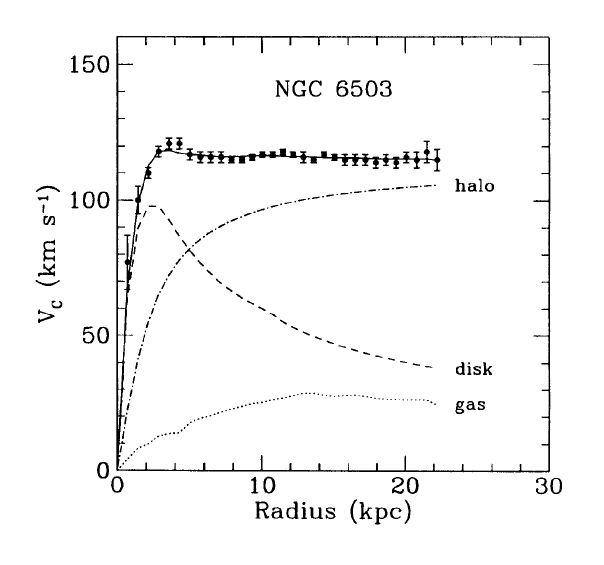
\includegraphics[width=0.4\textwidth]{DarkMatter/Rotationcurves}
\caption{Rotation curves of NGC 6503 galaxy. The image represents a fit on the rotation curves made of three parameters: a stellar (dashed) and a gaseous disk (dotted) and a Dark Matter halo (dash-dotted).}
\label{fig:rotation}
\end{figure}


\subsection{Cosmic Microwave Background}
The CMB is the residue of the thermal microwave radiation emitted \SI{\sim 3e5} years after the Big Bang, when the Universe became transparent to photons. Before that, the Universe was an ionized plasma in which matter and radiation were tightly coupled. It is a relic thermal radiation background which permeate the Universe and it is quite isotropic (\SI{2.73}{\K}). So CMB is a footprint of Universe at that moment from which several informations on cosmological parameters of that age can be inferred. One of them is the abundance of DM and Dark Energy. This result was achieved by analyzing the PLANCK experiment (ESA) measurements of the anisotropies of this radiation in universe. From a comparison between PLANCK results and the prediction of the cosmological model the Universe would be composed of ordinary matter for the 5\%, for Dark Matter for the 26\% and Dark Energy for the 69\% \cite{Planck:results}.

\section{The WIMP hypothesis}
\label{sec:wimp}
Dark Matter in the Universe is thermal relic of the Big Bang and its evolution can be summarized in a few different steps. Initially the early Universe was dense and hot, with temperature above the DM mass, and all particles were in thermal equilibrium: processes of annihilation and decay of DM and SM particles 
\begin{equation}
\chi\chi\longleftrightarrow \alpha\bar{\alpha}
\end{equation}
in which $\alpha$ is a generic SM particle and $\chi$ a generic DM candidate, happened in both directions. As the temperature of the Universe cool down, assuming that the mass of the WIMPs to be much higher than the one of the SM particles, the only interactions that occurred was:
\begin{equation}
\chi\chi\rightarrow \alpha\bar{\alpha}
\label{chitosm}
\end{equation}
because SM particles didn't have enough energy to create WIMPs pair.

Then the continuous expansion made DM particles to ``freeze out'' with their number asymptotically approaching a constant, their thermal relic density. DM particles become so dilute that they cannot find each other to annihilate. 

The whole process is described quantitatively by the Boltzmann equation:
\begin{equation}
\frac{dn}{dt}=-3Hn-\avg{\sigma_A v}\left(n^2-n_{\textup{eq}}^2\right)
\label{eqn:boltz}
\end{equation}
where $n$ is the number density of the DM particle, $H$ is the Hubble parameter, \avg{\sigma_A v} is the thermally averaged annihilation cross section, and $n_{\textup{eq}}$ is the DM number density in thermal equilibrium~\cite{feng:DM}. The first term on the right side of \Eqn{\ref{eqn:boltz}} represents the Universe expansion from which DM density decreases.The second one accounts for the annihilation and creation of DM interacting particles. The $n^2$ term arises from \Eqn{\ref{chitosm}} process that destroys $\chi$ in favor of SM particles and the $n_\textup{eq}$ arises from the opposite process which creates DM.

The term $n_\textup{eq}$ depends on the temperature $T$ of the Universe, it becomes Boltzmann suppressed by an exponential factor $e^{-m_\chi/T}$ and therefore approaches zero. The ``freeze-out'' time can be defined when $n\avg{\sigma_A v} = H$, i.e. when production cross section equals the expansion term. After that time the \Eqn{\ref{chitosm}} process becomes inhibited by the $H$ term so that even if it might occur again, DM particles are so far away from each other that it can't happen anymore.  

In this scenario the most reliable DM candidate is therefore a Weakly Interacting Mass Particle (WIMP). Indeed the ``WIMP miracle'' states that if such particle with mass \SI{\sim 100}{\gev} exists and it has a coupling $\sim \alpha$, i.e. interacts via weak force, and it is stable, it has a relic density consistent with the Dark Matter estimate, which is:
\begin{equation}
	\Omega_\textup{DM}h^2=0.1\left(\frac{0.01}{\alpha}\right)^2\left(\frac{m_\chi}{\SI{100}{\gev}}\right)
\end{equation}
\enlargethispage{1\baselineskip}
where $\Omega_\textup{DM}$ is the DM density and $m_\chi$ is the DM mass.

This implies that particles involved in the electroweak symmetry breaking, with mass in the \SI{10}{\GeV} - \SI{1}{\TeV} range, could be good candidate of DM and this allows to find the correct order of magnitude for the DM abundance \cite{DMcollider}.


%The freeze out occurs time when the $Hn$ term became important, i.e. $n\avg{\sigma_A v}= H$. At that time, the number density stopped changing and that is the relic abundance of Dark Matter we observe today.

%The relic density is therefore:
%\begin{equation}
%	\Omega_\textup{DM}=\frac{M_\textup{DM}n_0}{\rho_c}\simeq\frac{M_\textup{DM}T_0^3}{\rho_c M_\textup{Pl} T_f}\avg{\sigma_A v}^{-1}
%\end{equation}
%where $\rho_c=3H^2/8\pi$ is the critical density. So, the relic density is proportional to the inverse of annihilation cross section.

%\begin{figure}[pt]
%\centering
%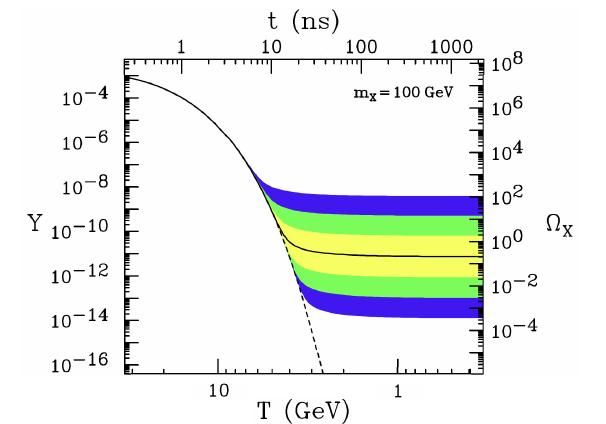
\includegraphics[width=0.75\textwidth]{DarkMatter/Freezeout}
%\caption{Evolution of WIMP number density (Y) and resulting thermal relic density (right) as a function of temperature T (bottom) and timet (top). The solid contour is for an annihilation cross section that yields the correct relic density, and the shaded regions are for cross sections that differr by 10, \SI{e2} and \SI{e3} from this value. The dashed contour is the number density of a particle that remains in thermal equilibrium. This image is taken from \cite{feng:DM}.}
%\label{fig:Freezeout}
%\end{figure}

Since WIMP DM candidates are particularly well-motivated, a robust experimental effort is underway to either discover DM, or constrain candidate theories. There are three main ways to detect DM which consist in the direct, indirect detection and production at colliders depending on wether the search is for DM candidates themselves or their annihilation products,

The direct detection consists in the search of WIMPs scattering from nuclei of ordinary matter. Since the nuclear recoil is very small, typically \SI{\sim 100}{\kev}, detectors capable of low energy detection thresholds, generally located underground, have to be built. The indirect detection consists in the search of the products of the annihilation processes that occur in the regions of the Universe where DM density is higher.

All the kind of detection methods are gathered in a Feynman diagram like in \Fig{\ref{fig:detection}}.

\section{Detection strategies}
\begin{figure}[pt]
\centering
{\fontfamily{pag}\selectfont  
\begin{tikzpicture}
	\draw[thick] (-3,1.5) -- (3,-1.5);
	\draw[thick] (-3,-1.5) -- (3,1.5);
	\filldraw[white] (0,0) circle (0.9cm) ;
	\filldraw[pattern=north east lines] (0,0) circle (0.9cm) ;
	
	\node[left] at (-3,1.5){DM};
	\node[left] at (-3,-1.5){DM};
	\node[right] at (3,1.5){SM};
	\node[right] at (3,-1.5){SM};
	
	\draw[draw=none, fill=orange!80!yellow!70] (-2.5,2)--(2.3,2) -- (2.3,2.2) -- (-2.5,2.2);
	\draw[draw=none, fill=orange!80!yellow!70] (2.2,1.8) -- (2.5,2.1) -- (2.2,2.4) --cycle;
	\node[] at (0,2.9){Indirect detection};
	\node[] at (0,2.5){(Thermal freeze-out)};
	
	\draw[draw=none, fill=yellow!80!red!50] (4,1.3)--(4,-1.1) -- (4.2,-1.1) -- (4.2,1.3);
	\draw[draw=none, fill=yellow!80!red!50] (3.8,-1) -- (4.1,-1.3) -- (4.4,-1) --cycle;
	\node[rotate=-90] at (4.6,0){Direct detection};
	
	\draw[draw=none, fill=orange!80!red!70] (-2.3,-2)--(2.5,-2) -- (2.5,-2.2) -- (-2.3,-2.2);
	\draw[draw=none, fill=orange!80!red!70] (-2.2,-1.8) -- (-2.5,-2.1) -- (-2.2,-2.4) --cycle;
	\node[] at (0,-2.6){Production at colliders};
	
\end{tikzpicture}
}
\caption{Feynman like diagram che ho fatto io which illustrates different methods for dark matter particle detection. The direction of the time axis selects a particular process. In indirect detection Standard Model (SM) particles coming from Dark Matter (DM) decays are revealed.  In direct detction the recoil of nuclei from DM scattering is measured. At colliders SM particles collide to produce a pair of DM candidate.}
\label{fig:detection}
\end{figure}
\subsection{Direct Detection}
The basic idea of Direct Detection is that if our galaxy is populated by WIMPs, a flux of them would run over our detectors and being detected. The WIMPs flux on the Earth is estimated to be of the order of \SI{e5}{\per \cm\squared\per\s}. The basic methodology for direct detection experiments is to look for this rare events that might be the signature of WIMP interactions, namely the elastic scattering of a WIMP on a target nucleus~\cite{snowmass}.

This kind of experiments must be carried out underground to reduce the signal contamination from every source of background. These sources come from cosmic rays, environmental radioactivity or detector radioactivity. For instance, two major experiments ongoing take place at LNGS, Italy, with the DAMA detector and followed by LIBRA, and in Modane, France, with the Edelweiss-III experiment at the LSM.
\begin{figure}[t]
\centering
\includegraphics[width=0.75\textwidth]{DarkMatter/damalibra}
\caption{Model-independent residual~\cite{damalibra} rate of the single-hit scintillation events, measured by the DAMA/LIBRA experiment in the \SIrange{2}{5}{\kev} energy intervals as a function of the time. The former DAMA experiment results are also shown. The zero of the time scale is January $1^{\text{st}}$ of the first year of data taking of the DAMA experiment. The superimposed curves represent the interpolated cosinusoidal function $A\cos{(t-t_0)}$. The dashed vertical lines indicate the maximum of the signal yield which occurs on June $2^{\text{nd}}$.}

\label{fig:damalibra}
\end{figure}

DAMA/LIBRA~\cite{damalibra} detector is made of 25 highly radio-pure \ce{NaI}, doped with Thallium, crystal scintillators assembled in a $5\times5$ matrix, whose main strategy is to measure WIMPs flux by looking at its eventual periodic variation. The periodic change in WIMPs relative velocity with respect to Earth orbiting around the Sun would lead to an annual modulation of the signal. Model independent results
%\footnote{i.e. measured rate of the single-hit events after subtracting the constant part $\avg{r_{ijk}-\text{flat}_{jk}}_{jk}$, where $r_{ijk}$ is the rate in the $i$-th time interval considered, for the $j$-th detector in the $k$-th energy bin and $\text{flat}_{jk}$ is the rate of the $j$-th detector in the $k$-th energy bin averaged over the annual cycles.}
, shown in \Fig{\ref{fig:damalibra}} for the interval \SIrange{2}{5}{\kev} in detected energy, actually show a modulation given by $A\cos{(t-t_0)}$ with period $T\simeq \SI{1}{year}$, a phase $t_0=\SI{152.2}{days}$ and an amplitude modulation $A =\SI{0.0204\pm0.0026}{counts/\kg/\keV}$. However DAMA/LIBRA results, covering a phase space region in which WIMP can be found shown in \Fig{\ref{fig:WIMPcs}}, are a bit controversial. Indeed, they are not confirmed by other experiments such the mentioned Edelweiss-III.

Interactions between WIMPs and nucleon can be spin-dependent when the sign of the scattering amplitude depends on the relative orientation of particle spins, or spin-independent when spin orientations do not affect the amplitude. For spin dependent interactions, the WIMP effectively couples to the net nuclear spin, due to cancellation between opposite spin pairs. It will differ whether the net nuclear spin is carried by a residual neutron or proton, see \Fig{\ref{fig:WIMPcsSD}}. The spin-independent interaction is expected to be coherent within the entire nucleus, so that if a WIMP has equal coupling to protons and neutrons, the rate scales with the square of the atomic mass of the target nucleus. 

Actual experiments only put upper-limits on WIMPs mass, which are summarized in \Fig{\ref{fig:WIMPcs}} for several experiments making any hypotheses on their nature.

\begin{figure}[p]
\centering
\subfloat[][Spin-Dependent WIMP-proton cross sections]
{\includegraphics[width=0.45\textwidth]{DarkMatter/spindepProtons}}\quad
\subfloat[][Spin-Dependent WIMP-neutrons cross sections]
{\includegraphics[width=0.45\textwidth]{DarkMatter/spindepNeutrons}}

\caption{Constraints on spin-Dependent WIMP-proton cross sections WIMP-neutron cross sections  as a function of WIMP
mass as of Summer 2013}
\label{fig:WIMPcsSD}
\end{figure}

\begin{figure}[p]
\centering
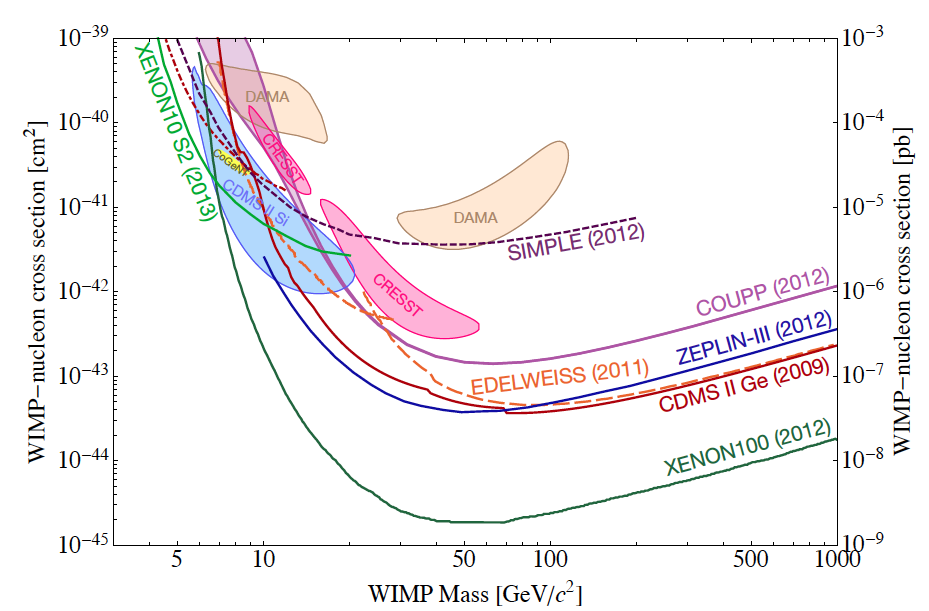
\includegraphics[width=0.75\textwidth]{DarkMatter/WIMPcs}
\caption{Constraints on spin-independent WIMP-nucleon cross section vs WIMP mass as of summer 2013.}
\label{fig:WIMPcs}
\end{figure}

\subsection{Indirect Detection}
The idea of Indirect Detection is to search for the products of the DM annihilation processes  happening in regions of the Universe where DM density is supposed to be higher like the center of the galaxy. Annihilation probability increases with DM density in a certain region of space and it produces SM particles such gamma rays, neutrinos, positrons, antiprotons. Therefore WIMPs can be detected by detecting these particles.

The disadvantage associated with Indirect Detection is the background induced by ``ordinary'' astrophysics. If considering only the signal strength from DM annihilations, the best target to detect annihilation products would be the galactic center, but there is a relatively unconstrained astrophysical background to any signals that could be produced there. Many research in the galactic center found signals consistent with DM annihilation but also compatible with the background and statistical fluctuations.

\subsection{Production at colliders}
The production at colliders share the same idea of direct detection: if a WIMP can scatter from a nucleon, it can be produced in \pp collision at high energy from annihilation of SM particles. Common to all collider DM searches is the signature of missing transverse momentum (\met) caused by the WIMPs escaping the detector. Therefore a striking proof of Dark Matter candidates production may be verified from an inbalance in the visible transverse momentum in the event.

Nevertheless we cannot tag \met as the only final state of a collision. Indeed, the experimental signature consists in a large value of \met and a back-to-back topology between \met and the Standard Model particle used for tagging the event, i.e in order to detect a possible WIMP, it must be associated with a detectable object. This kind of analyses are called \emph{Mono-X}. They are characterized by large missing transverse momentum and an energetic particle (the \emph{X}) such a jet (MonoJet), a photon (MonoPhoton) or a \Wboson or \Zboson boson (MonoV).

DM collider searches can be achieved in different ways. The first is to probe specific theories and models, and checking every decay channel predicted by a specific theory. This happens in every SUSY research for which every analysis is higly optimized for particular model. Another way is to reveal DM particles as the only accessible new state to an experiment.

%Once produced, DM will pass through the detector without leaving any tracks and without decaying into other particlese, as if it were a neutrino, since the iwe assumed that DM is weakly interacting and stable enough.

At the LHC, the MonoJet is the most sensitive search. On the other hand the \mph analysis, even if it works better at lepton colliders, at LHC provides good sensitivity and a very clean signature is achieved due to the request of a photon.

\section{The Minimal Dark Matter model}
The Minimal Dark Matter (DM) model~\cite{Cirelli:paper} extends the SM with a Electroweak (EW) fermion triplet, as a minimal candidate for WIMP DM. This candidate ($\chi$) is triplet under $SU(2)_L$, where the subscript L indicates coupling only to left-handed fermions, and singlet under color and hypercharge ($Y=0$). Its relevant Lagrangian is very simple and reads:
\begin{equation}
\begin{split}
\mathcal{L}_\chi&=\frac{1}{2}\bar{\chi}\left(i\slashed{D}-M_\chi\right)\chi \\
			&= \frac{1}{2}\bar{\chi_0}\left(i\slashed{\partial}-M_{\chi_0}\right)\chi_0+\bar{\chi}^+\left(i\slashed{\partial}-M_{\chi^\pm}\right)\chi^+ \\
			&+ g \left(\bar{\chi}^+\gamma_\mu\chi^+\left(s_w A_\mu + c_w Z_\mu \right) +\bar{\chi}^+ \gamma_\mu\chi_0W^-_\mu + \bar{\chi_0}\gamma_\mu\chi^+W^+_\mu \right)
\end{split}
\end{equation}
where $g$ is the $SU(2)$ gauge coupling, and $s_w$ and $c_w$ are the sine and the cosine of the Weinberg angle.

All the possible interactions between $\chi$ and other SM particles are required to preserve the gauge and the symmetries of the SM particularly the lepton number under which $\chi$ is assumed to be neutral. This last requirement is crucial, since it forbids the presence of higher dimensional operator that could lead a decay of $\chi$.  The difference at two loop level of $M_{\chi^\pm} - M_{\chi_0}$ is  about \SIrange{164}{165}{\mev}. This constrain was not applied to an eventual 5-plet particle which would have been automatically stable anyway. On the other hand the triplet has important features even beyond the DM motivation~\cite{Cirelli:paper} and it is capable to be produced at collider rather \mbox{than the 5-plet}.

If one requires that $\chi$ is thermally produced via the freeze-out mechanism discussed in \Sect{\ref{sec:wimp}}, and that it constitutes all the DM in the Universe, then we can estimate its mass to be \SIrange{3.0}{3.2}{\tev}. This range of mass, of course, is out of reach from LHC. Nevertheless for masses lower than \SI{3}{\tev}, $\chi$ is a subdominant DM component if thermally produced and its existence is again well justified to pursue any search at colliders. So, the Minimal DM model can be seen as a benchmark of the typical thermal-relic WIMP Dark Matter candidate, being a prototype for more complicated models, reproducing their low energy phenomenology with great accuracy.

As mentioned in the previous section, a way to search for WIMPs at colliders is via the so-called \emph{Mono-X} analyses. In this kind of searches the signal comes not only for the $\chi_0$ WIMP candidate particle but also from its two charged partners in the triplet. We can assume that the latter decay via a $\chi_0$ and soft, or low-momentum, charged pions (\pipm) both unreconstructed in the detector. 

A different, possible, scenario is that the tail of the decay distribution of the two charged $\chi$s might also leave tracks in the detector. These tracks would end when they decay as described into a couple of $\chi_0$ and charged pions. For that reason the \emph{disappearing tracks} would provide the most sensitive probe to the Minimal DM model, but also the most challenging from the experimental view perspective.

\smallskip
In this work a \mph analysis has been pursued following the lead of the one carried on in 2017 by the ATLAS Collaboration~\cite{paperMP}. In this context the \mph results were re-interpreted in terms of the Minimal Dark Matter model.










